\chapter{Magnetické převodovky}

Jak jsme v předchozí kapitole ukázali, přenášení momentu pomocí magnetů je možné a dokonce poměrně dobře prozkoumané. První patenty o přenosu momentu síly pomocí magnetů se objevily již na začátku 20. století \cite{patent}, ale kvůli technologickým nedostatkům doby byly brzy opuštěny. Teprve v posledních letech se díky pokrokům ve vědě opět objevuje zájem o magnetické převodovky.

% Výhody
Magnetické převodovky byly dříve zavrhnuty kvůli mnohým nedostatkům:

\begin{enumerate}[topsep=0pt, partopsep=0pt]
    \setlength{\itemsep}{0pt}%
    \setlength{\parskip}{0pt}%
    \item Maximální přenositelný moment síly je malý.
    \item Složitá konstrukce.
    \item Potřeba silných magnetických materiálů a materiálů s vysokou permeabilitou.
    \item Nedostatek využití, kde by mechanické převody nefungovaly lépe.
\end{enumerate}

V dnešní době se však objevují nové situace, ve kterých jsou magnetické převodovky dobrým řešením. Jako příklad uvedeme jejich použití ve vesmíru. Magnetické převodovky totiž dobře odolávají nízkým teplotám \cite{NASA_MG} narozdíl od standarní lubrikačních látky, které jsou potřebné k běhu mechanických převodů. Nejvýznamnějšími výhodami magnetickým převodovek jsou:

\begin{enumerate}[topsep=0pt, partopsep=0pt]
    \setlength{\itemsep}{0pt}%
    \setlength{\parskip}{0pt}%
    \item Srovnatelná objemová hustota momentu síly magnetických a mechanických převodovek \cite{torque_dens}.
    \item Využití, ve kterých mechanické převodovky nemohou být použity.
    \item Minimalní tepelné ztráty.
    \item Nizká či nulová údržba a možnost používání bez lubrikace.
    \item Automatická ochrana proti přetížení.
    \item Kompaktnost a možnost slučovat více magnetických systémů do jednoho celku \cite{MT_full}.
    \item Možnost nahradit mnohé druhy mechanických převodů.
    \item Odolnost proti písku a jiným nečistotám.
    \item Možnost použití ve vakuu bez potřeby odplynění maziv.
\end{enumerate}

\clearpage

\begin{wrapfigure}{r}{0.50\textwidth}
    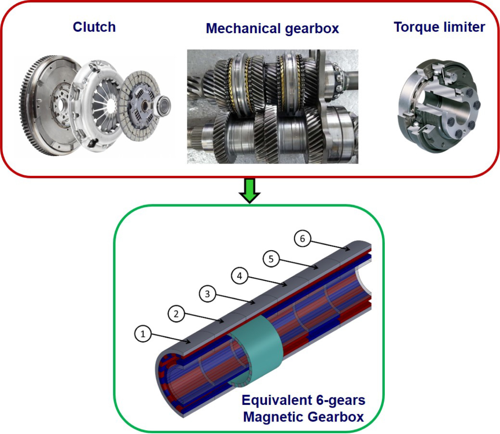
\includegraphics[width=0.45\textwidth]{magnetic_transmission.png}
    \centering
    \caption{Nákres šestistupňové magnetické převodovky (zdroj: \cite{MT_full}).}
    \label{fig:magnetic_transmission}

    \vspace{1cm}

    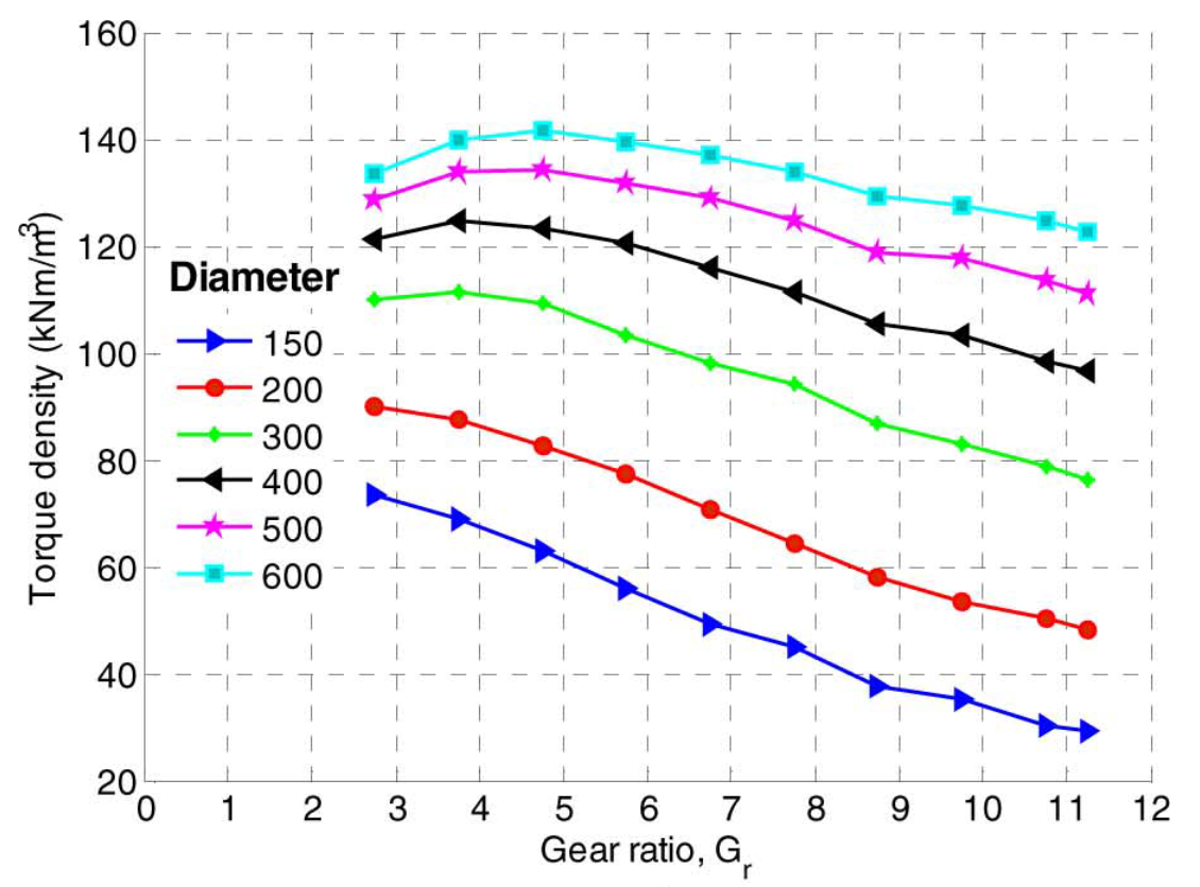
\includegraphics[width=0.45\textwidth]{torque_density_mag.png}
    \centering
    \caption{Hustota momentu síly referenčních magnetických převodovek (zdroj: \cite{torque_dens}).}
    \label{fig:torque_density_mag}

    \vspace{1cm}

    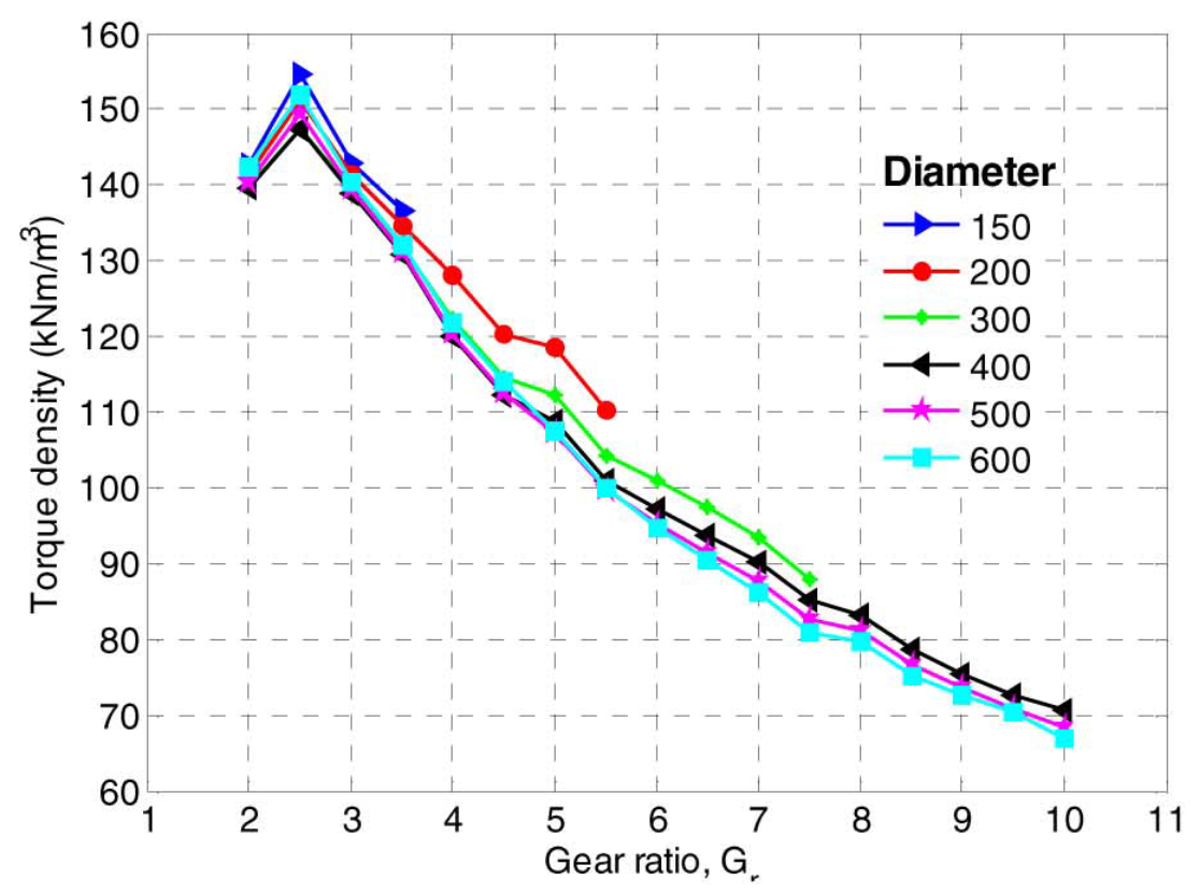
\includegraphics[width=0.45\textwidth]{torque_density_mech.png}
    \centering
    \caption{Hustota momentu síly referenčních mechanických převodovek (zdroj: \cite{torque_dens}).}
    \label{fig:torque_density_mech}
\end{wrapfigure}

\subsection{Kompaktnost}
Dříve zmíněná kompaktnost magnetických převodovek spočívá ve spojení funkcí spojky, převodovky a momentového omezovače v jednom. Posouváním modulátoru po délce převodovky, která je rozdělena na 6 částí s různým počtem pólových párů, jsme schopni vybírat převod. Zároveň s tím magnety plní funkci spojky a momentového omezovače, protože při překonání maximálního momentu síly kolem sebe prostě proklouznou a znovu se zapojí až na dalším "mgnetickém zubu". Návrh takové převodovky je k vidění na obrázku \ref{fig:magnetic_transmission}.

\subsection{Hustota momentu síly}
K porovnávání kvality převodovek je často používána míra momentu síly, který dokáže daný návrh přenášet, v závislosti na jejich objemu nebo hmotnosti. Při dopravě zařízení do vesmíru může právě objem nebo hmotnost hrát klíčovou roli v tom, zda bude zařízení použito. V grafech \ref{fig:torque_density_mag} a \ref{fig:torque_density_mech} je vidět porovnání hustot momentu síly magneticckých a mechanických převodovek v závislosti na jejich průměru a převodovém poměru.

\subsection{Druhy magnetických převodů}
Pricip magnetických převodů vychází ze schopnosti vytvořit pomyslný "magnetický zub", který nahrazuje klasické zuby v ozubených kolech. Rapidní vývoj silnějších a odolnějších magnetických látek dovoluje vytvářet nejrůznější konfigurace magnetických převodů a inspirovat se jejich mechanickými protějšky. Na obrázku \ref{fig:topologies_simple} jsou k vidění různé topologie magnetických převodů a jim odpovídajících mechanických ekvivalentů.
\begin{wrapfigure}{r}{0.50\textwidth}
    \vspace{-5cm}
    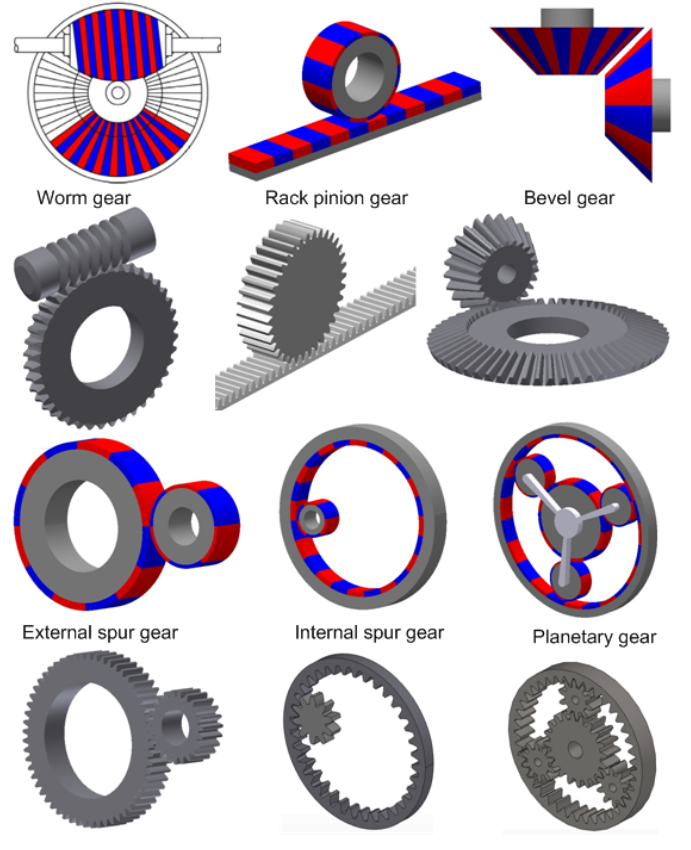
\includegraphics[width=0.45\textwidth]{simple_gears.png}
    \centering
    \caption{Základní magnetické topologie a jejich mechanické ekvivalenty (zdroj: \cite{MG_topologies}).}
    \label{fig:topologies_simple}
\end{wrapfigure}

Více pozornosti je však věnováno hlavně převodovkám s vyšší momentovou hustotou (planetární a harmonické) nebo jinou složitější topologií (koncentrické) (viz \autoref{fig:topologies_complex}).

Kromě topologie je také zájmem zkoumání orientace jednotlivých magnetů. Zde je dobré zmínit orientaci zvanou Halbachovo pole\footnote{Halbachovo pole (anglicky \textit{"Halbach array"}) je speciální uspořádání, jehož planární varianta se snaží o minimalizaci unikajicího pole z jedné strany.}.
\begin{figure}[H]
    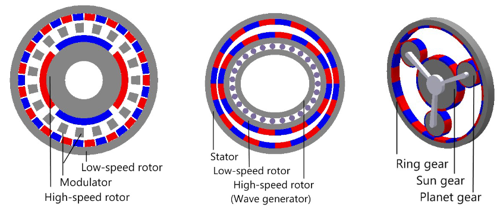
\includegraphics[width=0.45\textwidth]{torqe_dense_gears.png}
    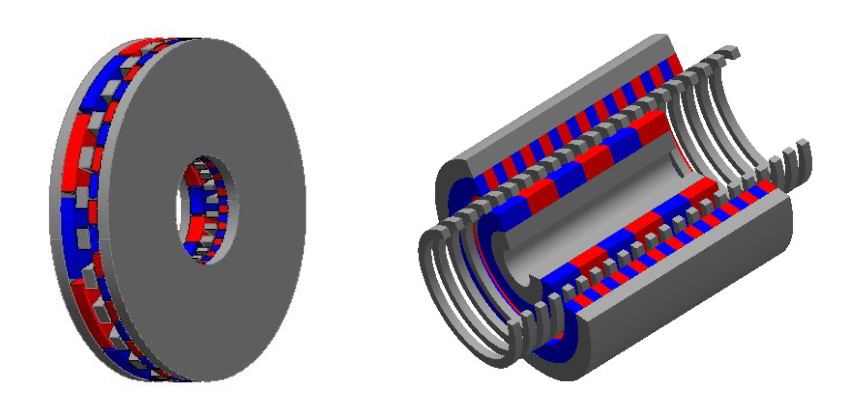
\includegraphics[width=0.45\textwidth]{concentric_gears.png}
    \centering
    \caption{Příklady magnetických převodů s vyšší hustotou momentu síly (první 3 zleva) a koncentrických převodů (první 2 zprava) (zdroj: \cite{MG_topologies}).}
    \label{fig:topologies_complex}
\end{figure}

\section{Vlastní návrhy}

% jaký jsme si vybrali způsob

\subsection{Princip fungování}

\subsection{První návrh}

% 3D design

% zhodnocení / ponaučení

\subsection{Druhý návrh}

% 3D design

% \subsection{Měření}
% Měření plechů